\section{Results}
\subsection*{Bayesian Model}

Diagnostic plots for Bayesian model fit to the real apixaban data is shown in \cref{fig:fig3}.  Posterior population prediction intervals (that is, the result of integrating out the random effect of each patient) of the observed concentration are realistic and to the eye appear similar to the observed data (top left of \cref{fig:fig3}).  Residual plots (observed minus posterior mean) indicate homogeneity of variance on the log scale, which is consistent both with expert knowledge on the measurement process and the likelihood we choose (bottom left of \cref{fig:fig3}). Predicted concentrations tend to agree with observed concentrations (top right of \cref{fig:fig3}), and posterior predictive draws have similar empirical cumulative distribution functions as the observed data (bottom right of \cref{fig:fig3} ). In \cref{fig:fig4}, we show concentration functions obtained from draws from our prior distribution as well as two patients with best and worst fit as measured by mean absolute percent error (best: 3.29\%, worst: 26.4\%). Because our HMC diagnostics do not indicate problematic behaviour in the Markov chains, and because the model diagnostics indicate adequate fit, we believe the obtained model’s posterior predictive distribution is adequate for simulation of pseudodata.


\begin{figure}
	\centering
	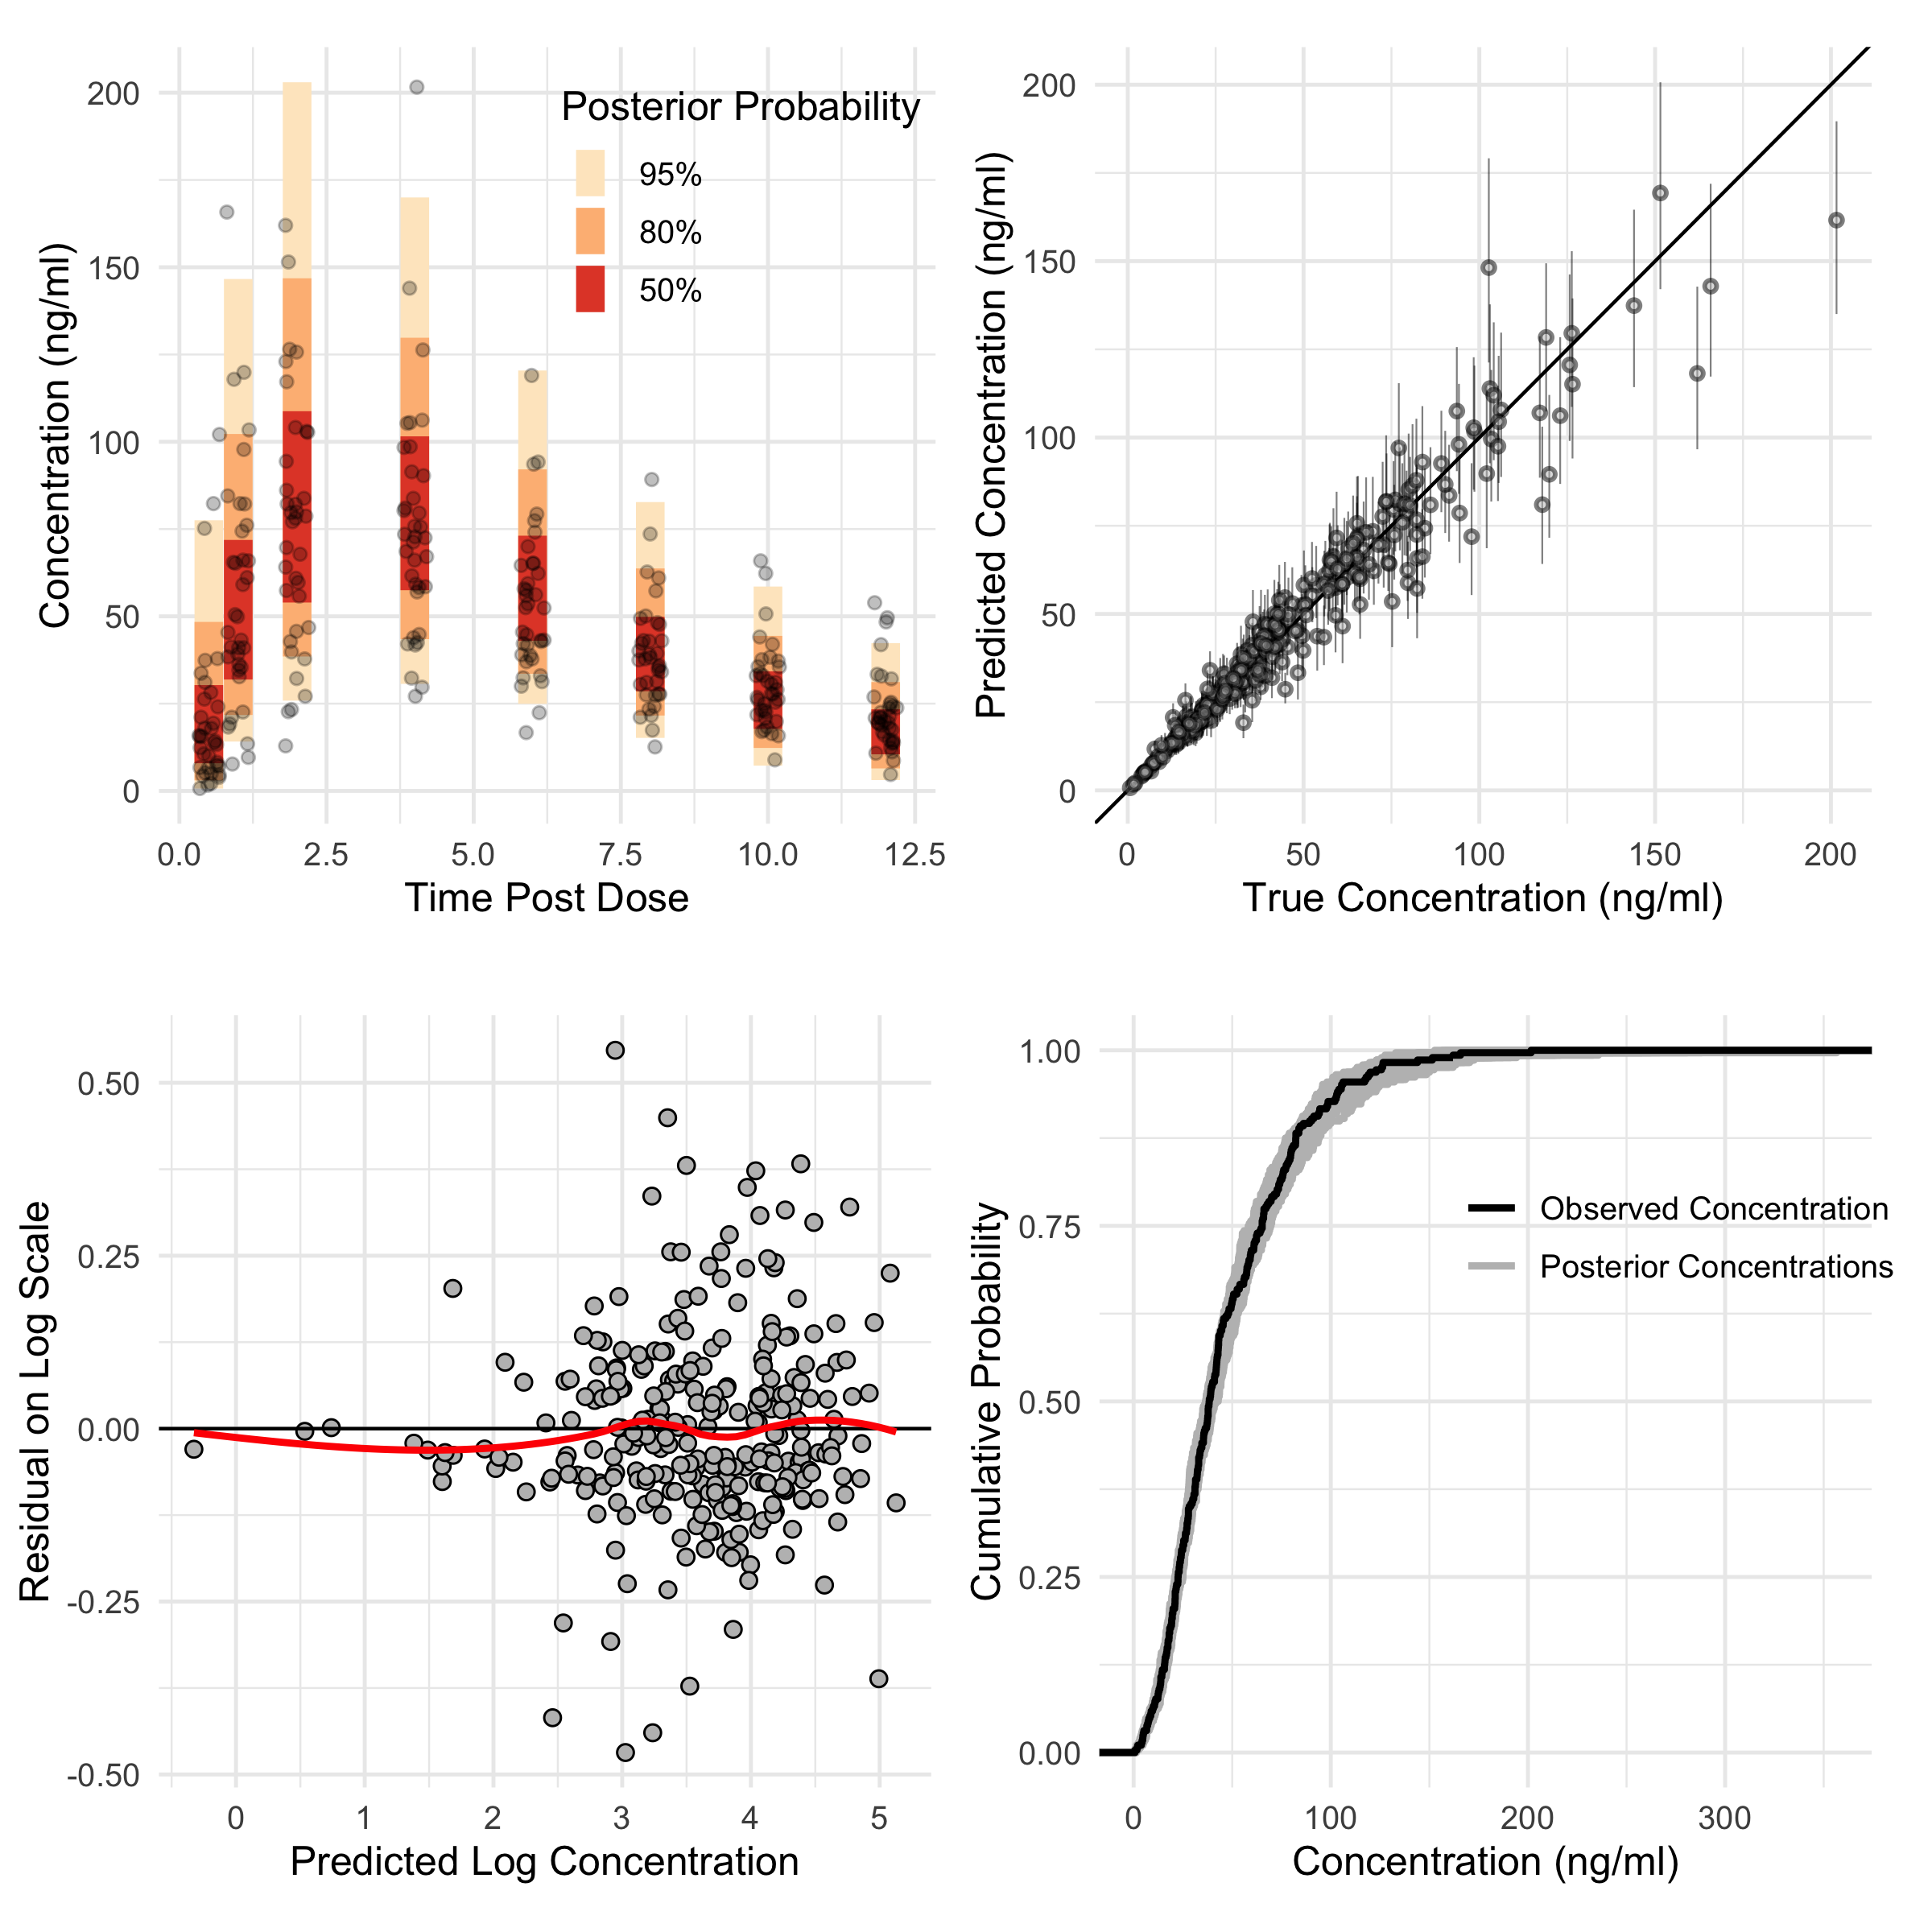
\includegraphics[width=0.9\linewidth]{figs/diagnostics}
	\caption{Diagnostic plots for our Bayesian model.  Top left shows the posterior predictive distribution plus observed data.  Data points gave been perturbed to prevent overlapping. Top right shows the predicted values along with accompanying 95\% equal-tailed posterior credible interval. Bottom left shows the residuals (on the log scale) between the observed concentrations and the posterior mean concentration, bottom right shows the cumulative density function for the observed data (black) as well as draws from the posterior predictive distribution (gray).}
	\label{fig:fig3}
\end{figure}


\begin{figure}
	\centering
	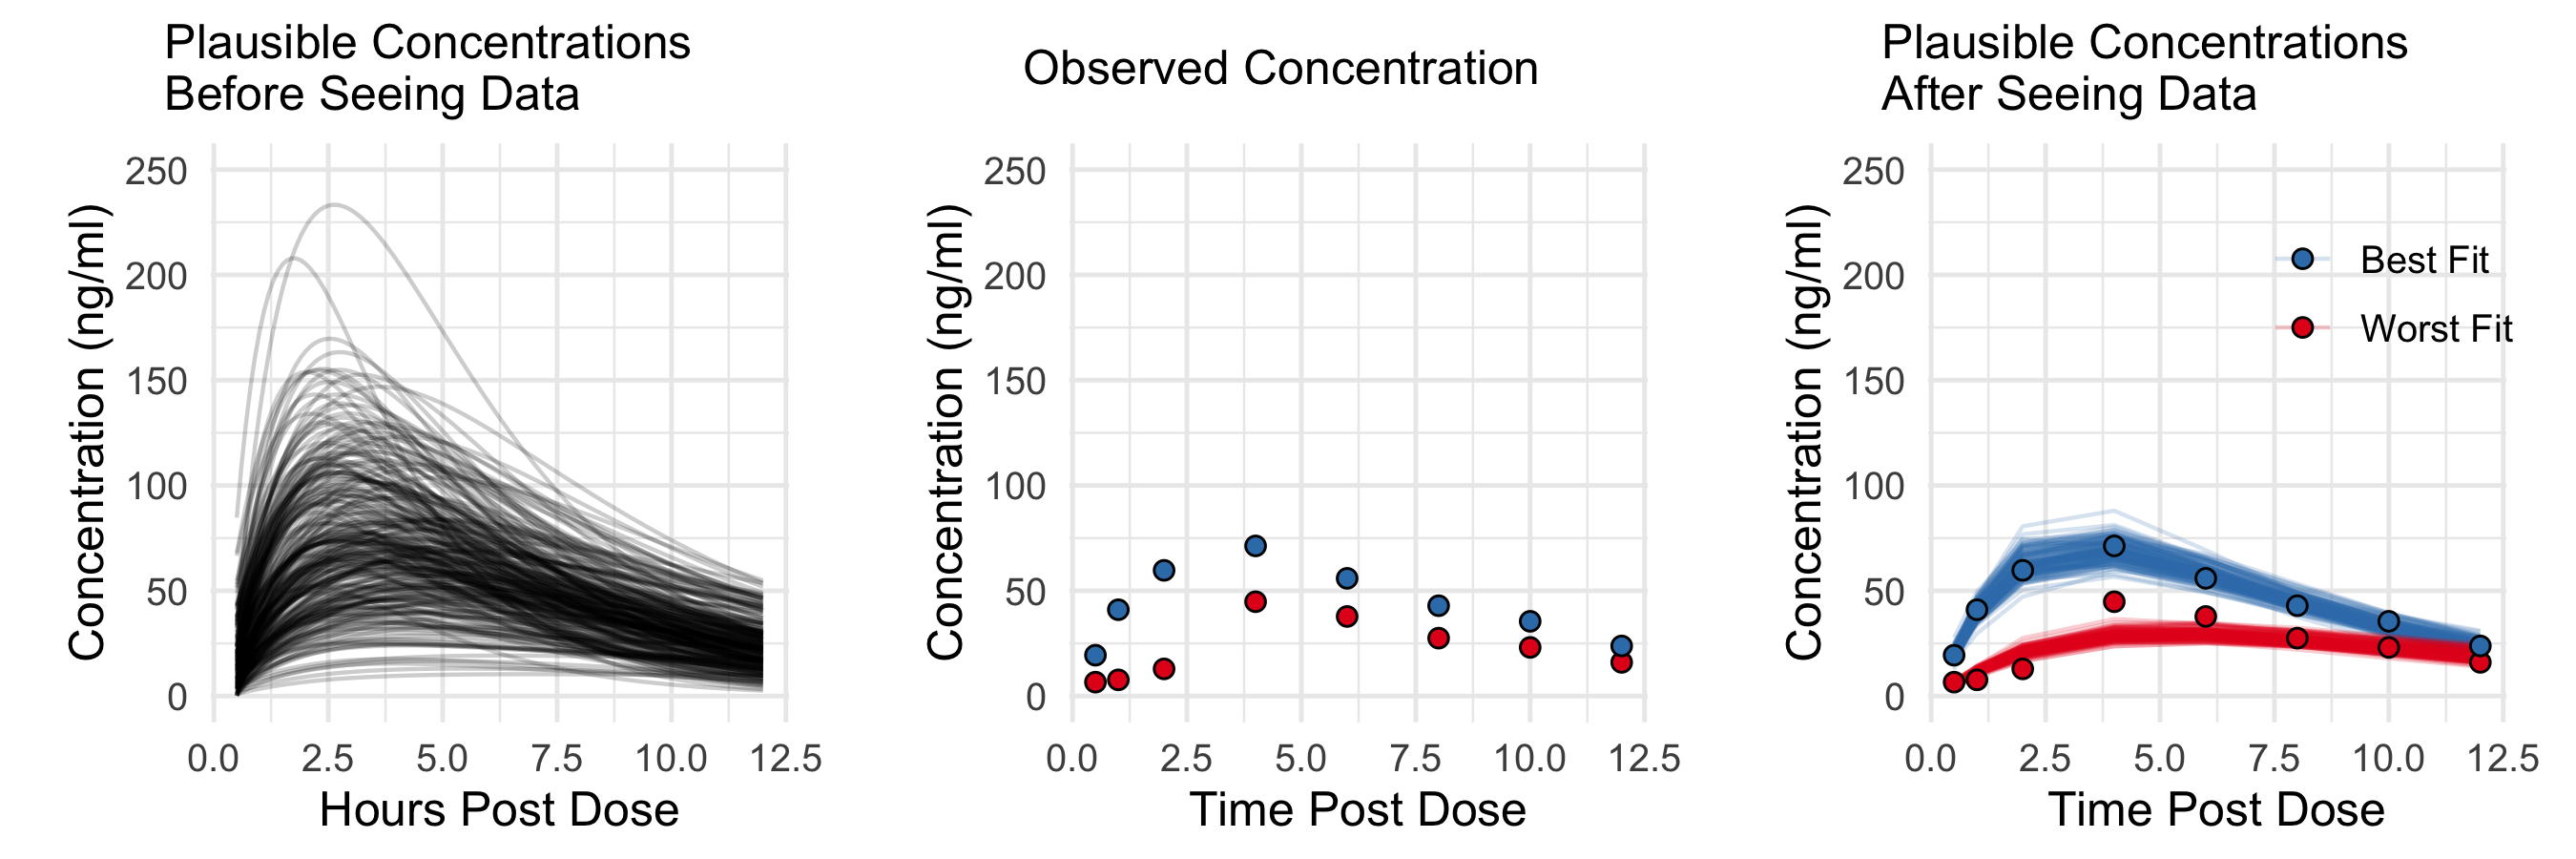
\includegraphics[width=\linewidth]{figs/fig3}
	\caption{The leftmost panel shows 250 draws from the prior defined in the previous section.  The center panel shows data from two patients who acieved the best (blue) and worst (red) model fit as measured through mean absolute percent error.  The rightmost panel shows 250 draws from the posterior for these patients.  Not shown here are the other 34 patients in our data, for which the model is also capable of performing predictions for. }
	\label{fig:fig4}
\end{figure}


\subsection*{Fit on Simulated Patients Using HMC and MAP}

Initial comparisons of predicted values indicate that both HMC and MAP yield similar predictions to one another, and similar predictions to actual values of unseen data.  Examining predictions alone, it would seem that HMC and MAP are equivalent, or at the very least similar enough so as to not have strong preference for one over the other. When using posterior means, HMC results in lower prediction error on unseen data as measured with Root Mean Squared Error (RMSE), Mean Absolute Error (MAE), and Mean Absolute Percentage Error (MAPE), but these are not stark differences. Estimates of posterior uncertainty between MAP and HMC can however vary a great deal. Shown in \cref{fig:fig6} are 18 of the 100 simulated patients which have a MAP equal tailed posterior interval at least 50\% larger as compared to their HMC equal tail posterior interval at the widest point. We note that while not shown explicitly, unobserved concentrations lie entirely within the HMC and MAP posterior intervals.

\begin{figure}
	\centering
	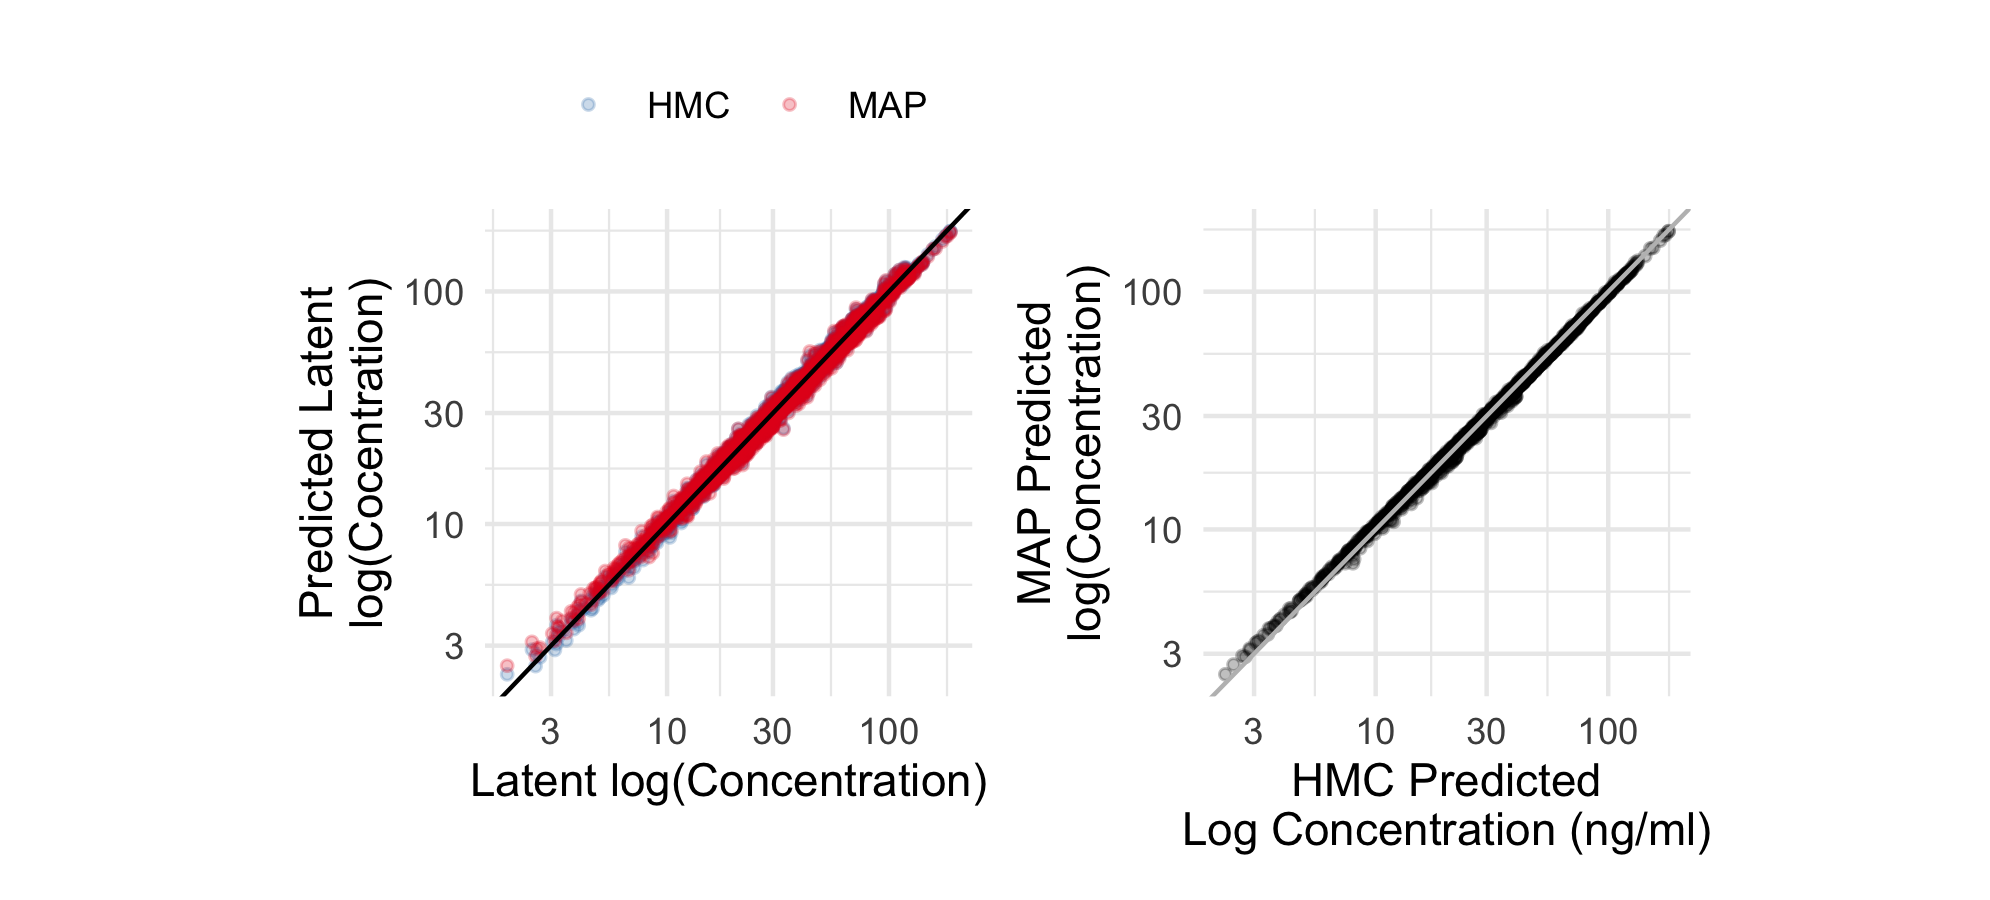
\includegraphics[width=0.85\linewidth]{figs/compare}
	\caption{Comparisons of fits obtained through HMC and MAP for simulated patients.  On the left, the two methods are compared to the true concentration values, and on the right the two methods are compared to one another.  The predictions are negligibly different to the eye and are also negligibly different as compared by Root Mean Squared Error (RMSE), Mean Absolute Error (MAE), and Mean Absolute Percentage Error (MAPE).}
	\label{fig:fig5}
\end{figure}


\begin{table}
	\centering
\begin{tabular}{|c|c|c|}
	\hline 
	& HMC & MAP \\ 
	\hline 
	RMSE & 3.52 & 3.99 \\ 
	\hline 
	MAE & 2.35 & 2.72 \\ 
	\hline 
	MAPE & 0.04 & 0.05 \\ 
	\hline 
\end{tabular} 
\caption{Comparison of HMC and MAP on three loss functions common in pharmacokinetics: Root Mean Squared Error (RMSE), Mean Absolute Error (MAE), and Mean Absolute Percentage Error (MAPE). \textbf{Could present standard deviations of these? Let's discuss.}}
\end{table}

\begin{figure}
	\centering
	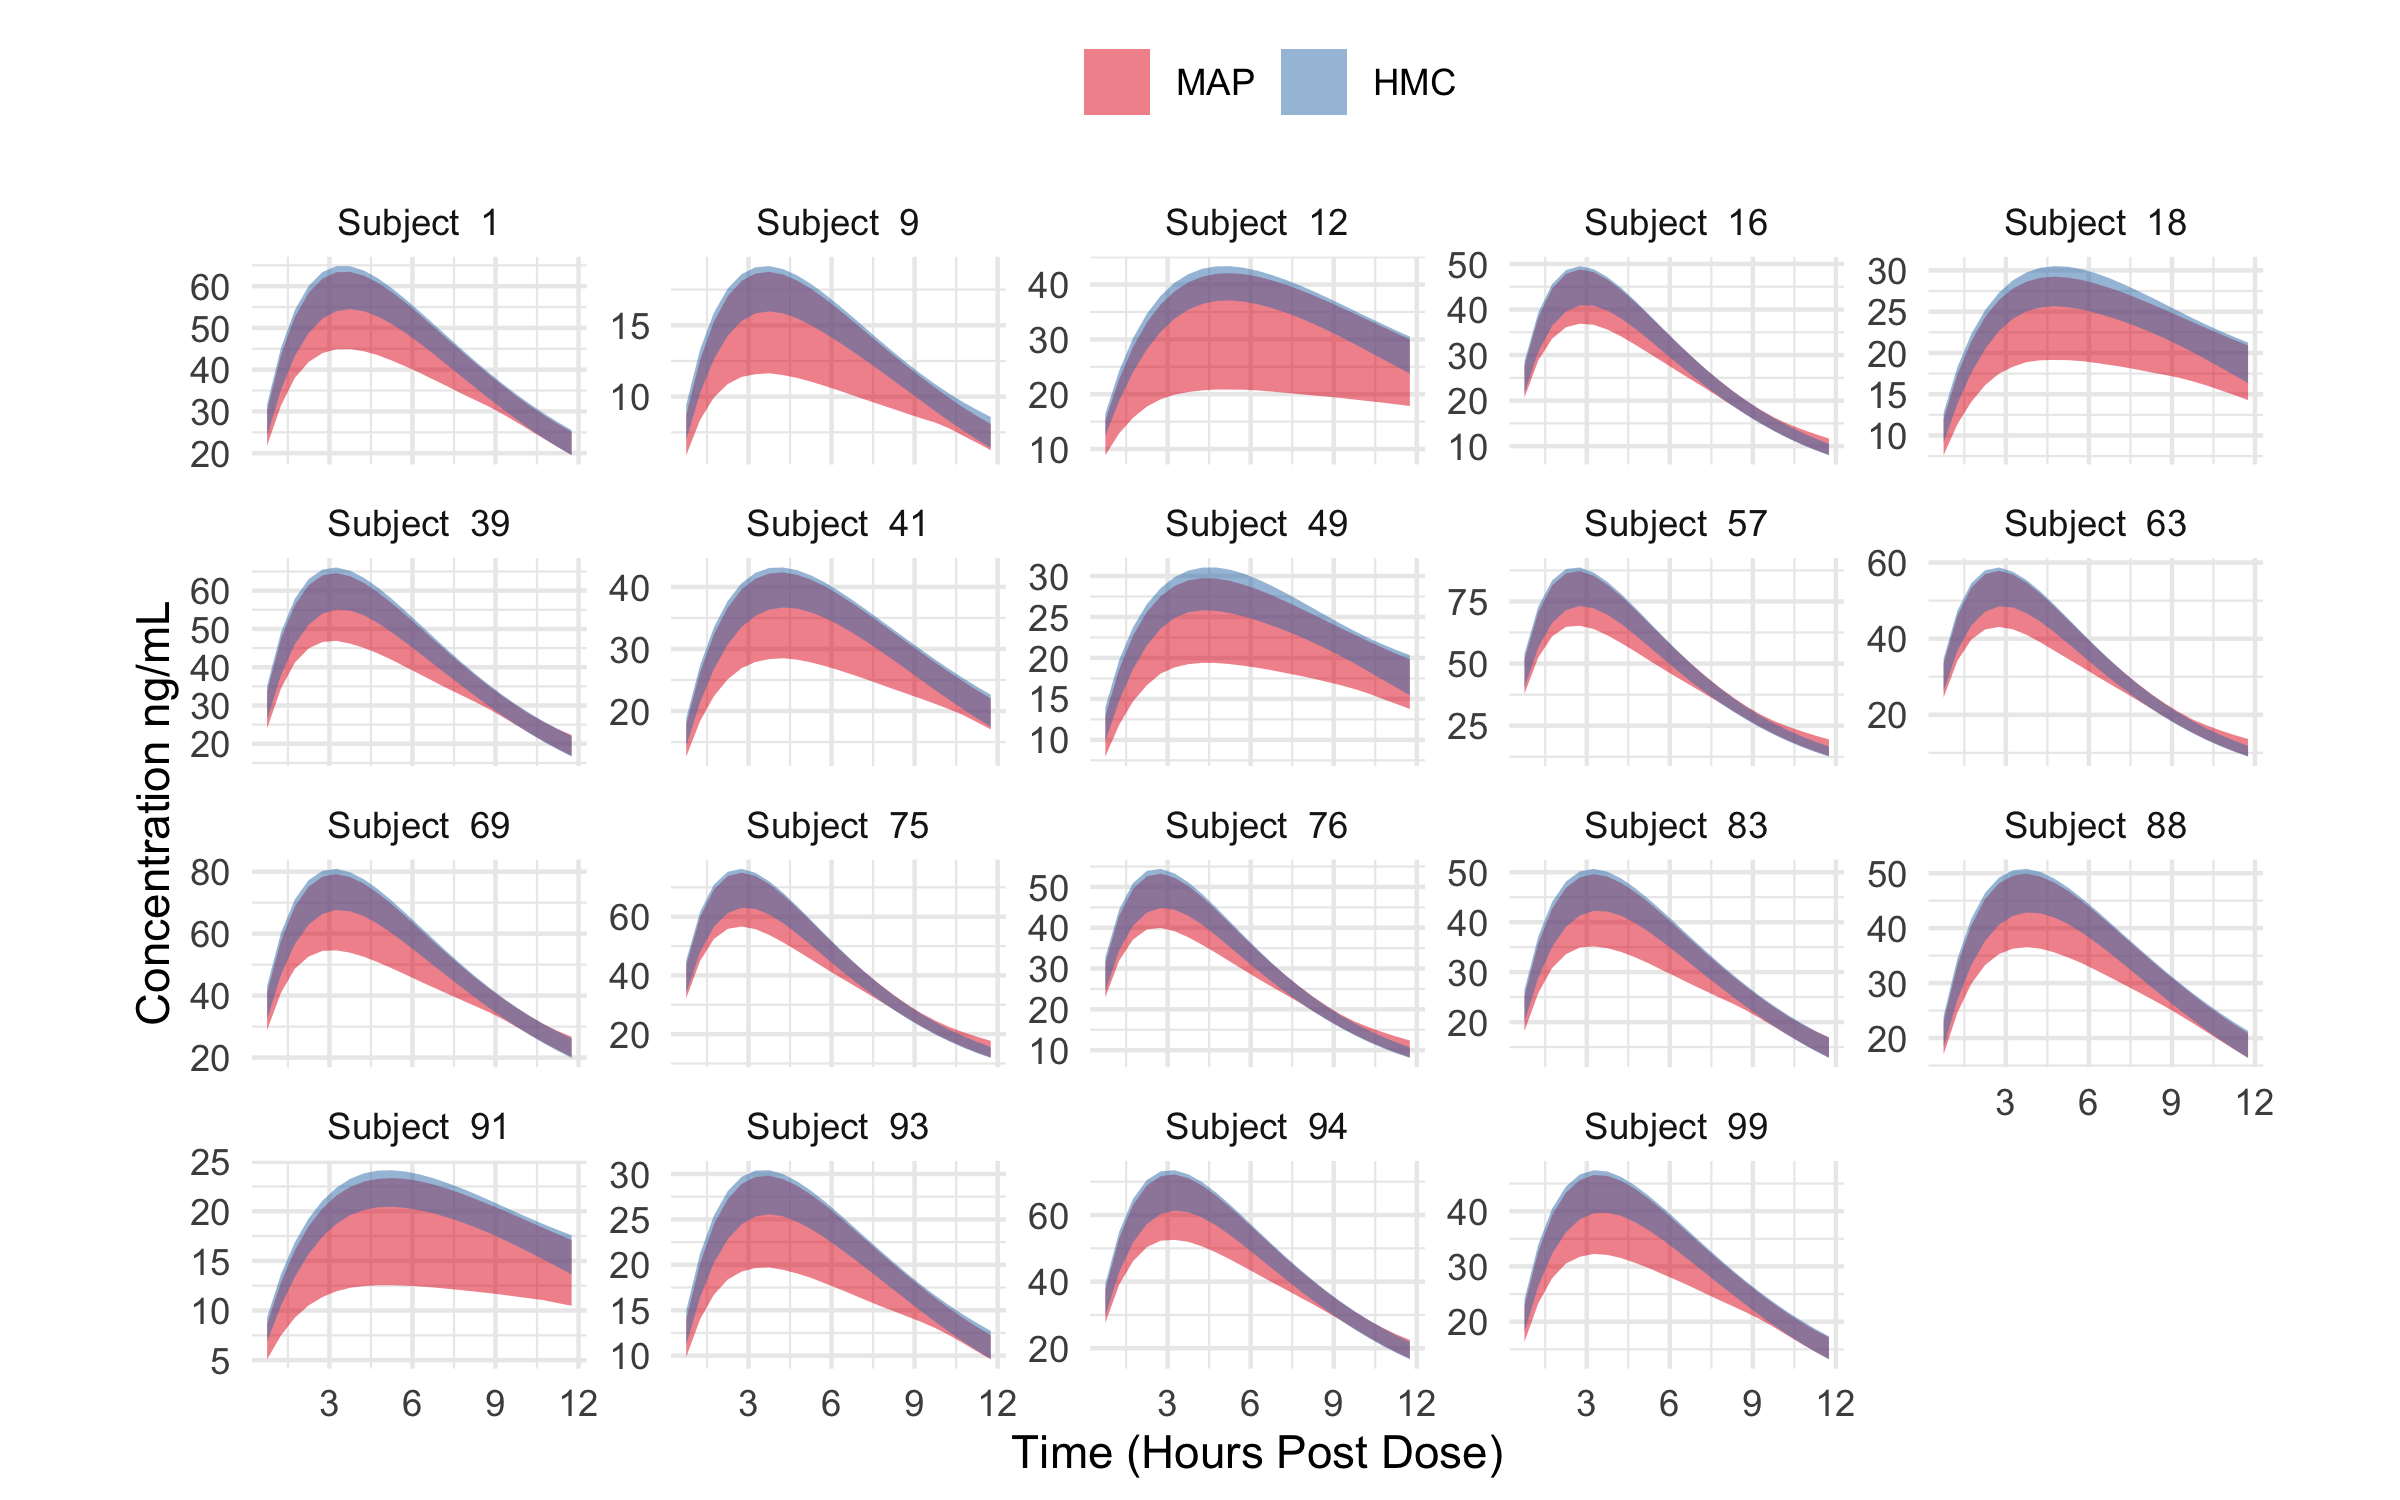
\includegraphics[width=1\linewidth]{figs/intervals}
	\caption{Comparisons of equal tail posterior intervals from MAP and HMC. Note that the concentration scales differ from subplot to subplot.  Selected patients are those which have a MAP posterior interval at least 50\% as wide or wider than their HMC interval.  In many simulated subjects.}
	\label{fig:fig6}
\end{figure}


\subsection*{Difference in Estimated Dose To Achieve Target Risk}


Shown in \cref{fig:fig7} are the differences between doses computed from HMC and MAP posteriors to achieve the indicated level of risk.  The left panel shows the difference in doses in order to achieve a concentration of at least 20 ng/ml 12 hours post dose. For a majority of patients, MAP and HMC agree to within 1 mg though some pseudopatients see a much larger dose recommendation by HMC than by MAP.  An increase in dose size will always lead to a smaller risk, and so as the dose size increases the differences tend to 0, though the two methods never perfectly agree.

The right panel shows the difference in doses in order to spend no more than the indicated proportion of the 12 hour observation period below 20 ng/ml (we call this an “acceptable risk”).  Small dose sizes lead to large risks in this experiment.  Both MAP and HMC tend to agree to within 0.5 mg.  As the acceptable risk decreases, dose sizes tend to diverge, with MAP recommending larger doses for the majority of pseudopatients.

\begin{figure}
	\centering
	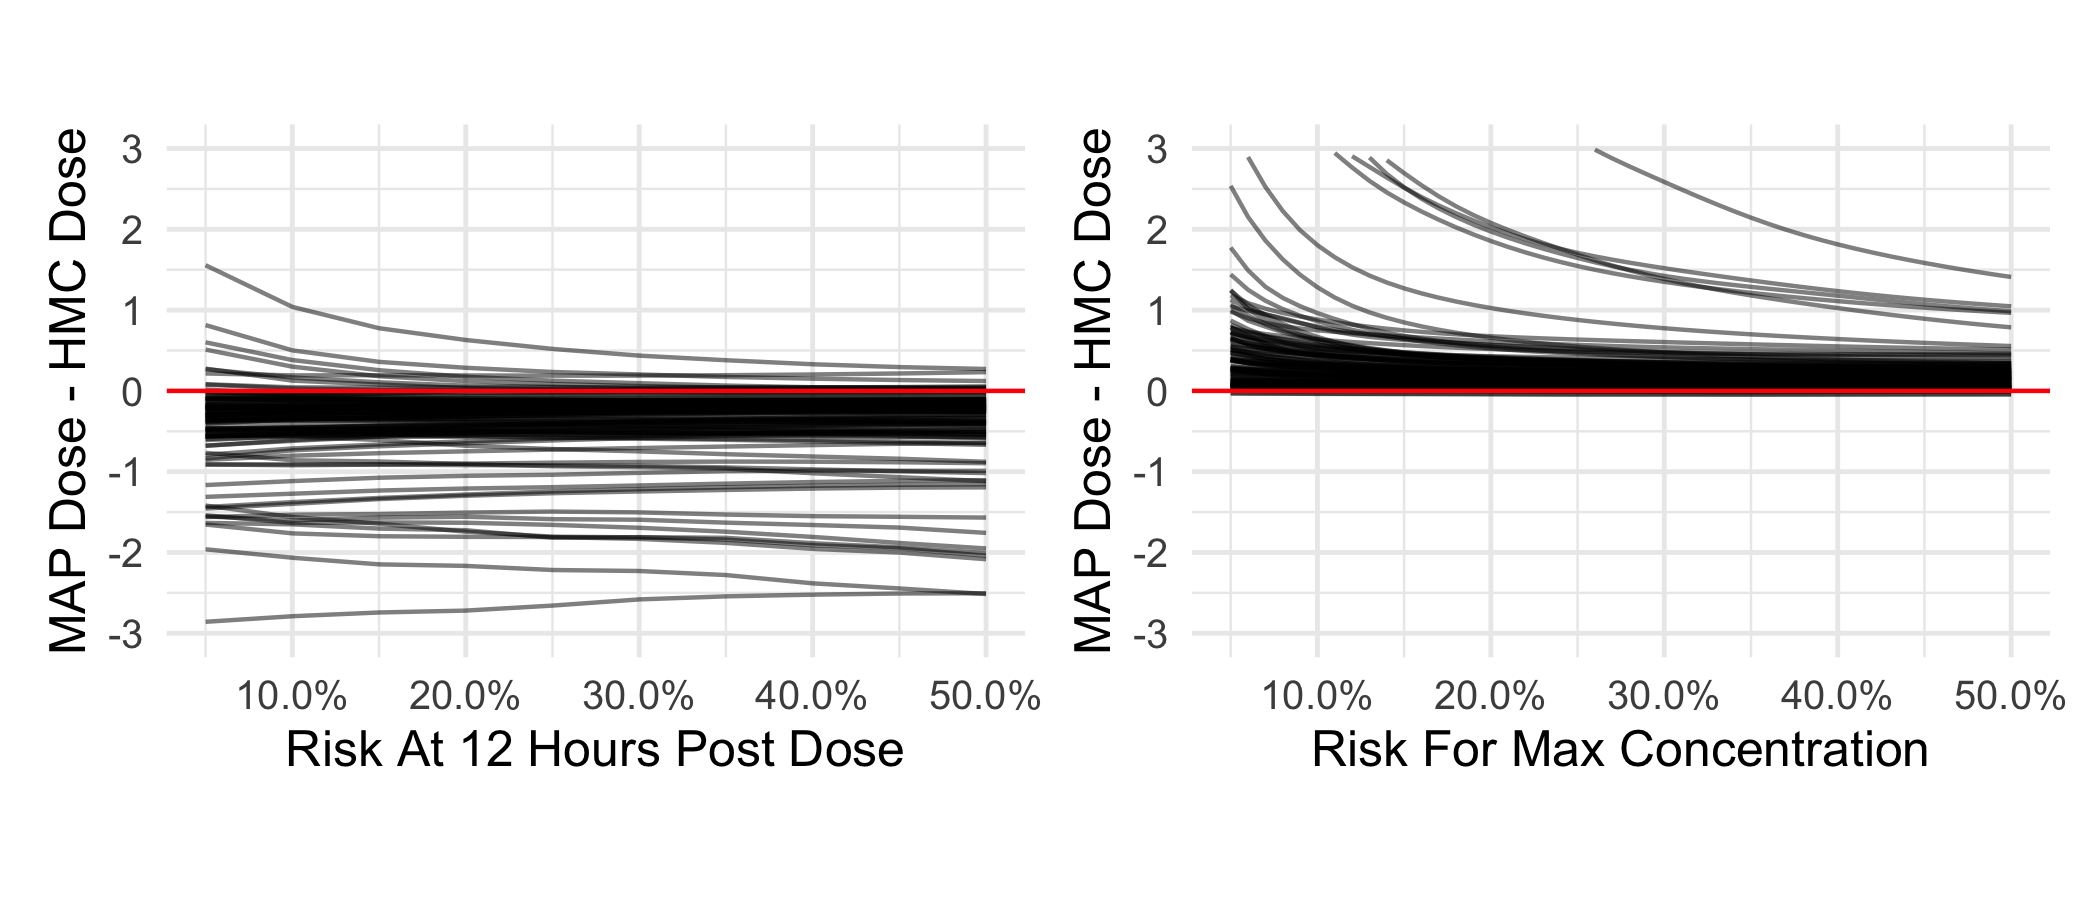
\includegraphics[width=\linewidth]{figs/experiments}
	\caption{Left: Differences between the estimated doses from MAP and HMC to achieve the indicated risk of having a concentration of apixiban smaller than 20 ng/ml at 12 hours post dose. Right: Differences between estimated doses from MAP and HMC to achieve the indicated risk of being below 20 ng/ml over the 12 hour observation period.}
	\label{fig:fig7}
\end{figure}



